
% status: 85
% chapter: TBD

\title{Twitter Sentimental Analysis with Spark}


\author{Venkatesh Aditya Kaveripakam}
\affiliation{%
\institution{Indiana University}
\city{Bloomington}
\state{IN}
\postcode{47408}
\country{USA}}
\email{vekave@iu.edu}

\author{Surya Prakash Sekar}
\affiliation{%
\institution{Indiana University}
\city{Bloomington}
\state{IN}
\postcode{47408}
\country{USA}}
\email{sursekar@iu.edu}

% The default list of authors is too long for headers}
\renewcommand{\shortauthors}{Aditya}{Surya}

\begin{abstract}

In this project we have built a RESTful webservice that will accept a topic of 
interest as input from the user which is the twitter hashtag in this case and 
query the relevant hashtag data from the twitter API using tweepy package from 
python and making use of its cursors. All pre-processing and data cleaning 
involved with the tweets data will be handled in python using a variety of 
tweet pre-processing techniques and a consumable dataset for spark is created. A 
sentimental analysis model is created using python's textblob as well in order to label 
the tweets before in hand for the hashtag data that is selected by the user. 
SparkML library is then used to perform sentimental analysis on the tweets data 
and a summary is provided with respect to it. A graph displaying the 
distribution of the tweets based on the sentiment and the top 5 positive and 
negative tweets with respect to the input hashtag is also displayed.

\end{abstract}

\keywords{hid-sp18-411,hid-sp18-418, Swagger, Spark, API, Cloud, Twitter}

\section{Introduction}

A lot of research related to social media data would provide a relevant guide on how 
social media data can be used in research, by the inherent dynamism in society 
instantaneously reflected in social media demands a breakaway from the traditional 
process of academic publishing. This is true of many fields, but is especially relevant 
when we consider the immediacy and mutability of social media data. In order to 
truly capture the potential of social media, we need to explore methods of conducting 
and disseminating research that can keep up with the pace of modern life. Data in 
social media represents users behavior, attitudes, feelings, views and relationships are
increasingly being re-used for research purposes in in both academia and industry. 
Even though social media has entered the deeper circle of our culture, we must 
not overlook the fact that social media is driven by the people of our society. 
So, it is very much likely that the posts can be simulated to get the desired 
results. Such kind of methods not only brute force their way through the 
algorithm, but also indirectly manipulate the human mind. Hence, we
should be very careful when we are analyzing social media data for prediction 
and should take into consideration the above-mentioned issues while they are 
conducting the research.

With millions of users and thousands of tweets every second worldwide, enormous 
data is publicly available with Twitter that can be used for various research purposes. 
Twitter is one of the best places for breaking news because of it’s unique 
small-size story sharing and re-tweeting options. Tobias Preis shows how 
Twitter feed can be used to know the most recent updates about companies or 
major incidents to predict the stock price~\cite{hid-sp18-418-effect-twitter}. 
It is also well known that using certain words in speech can attract a lot of attention 
either positive or negative. Some amazing features of twitter are retweeting and 
favoriting that helps people support a person’s idea through showing their 
approval for it. We utilize some of these features from twitter to analyze what are the 
different words that have been used with respect to a hashtag that gained a lot of 
attention from public and led to a huge population participate in the trend. 
Our research in this project is mostly focused on understanding the different 
words around the tweets that have gained a lot of attention from public and also 
showing how the regular sentiment analysis might be very useful to understand 
people’s opinion on it. By showcasing the top positive and negative tweets and 
the split of the tweets based on sentiment, we would be able to get a overall 
picture with respect to an issue. For example, lets consider that our favorite 
football team is playing a game, then using a relevant hashtag we would be able 
to visualize the emotions of the general public over the course of the game, and 
results would ideally be something like where if the team wins then the output 
would be a lot of positive tweets in contrast to negative and neutral tweets. 


\section{Sentimental Analysis}
Sentiment analysis is a contextual mining that extracts the sentiments hidden in 
the sentences. Sentiment analysis is extremely useful in social media research as 
it allows us to gain an overview of the wider public opinion behind certain topics.
This technique is majorly used in the social media streams to understand how people 
are reacting to a situation or product or brand. This is very helpful in the 
marketing area where words that have more public approval 
can be identified and utilized in the marketing of a product or brand. Many 
sentiment analyses generally classify a sentence into one of different buckets 
like positive or negative of neutral. To make this classification, there needs 
to be a dictionary of words for each of these categories which are treated as 
positive or negative or neutral. To understand the sentiment in a tweet or a 
sentence, based on the number of positive words and number of words that belong 
to any particular category it contains, will be given a score. Based on the 
score, the sentence is then classified into positive or negative or neutral. 
There are some pre-defined libraries with words in these categories readily 
available to use for most of the situations. It is generally a good practice to 
manually tag some tweets as positive and negative and then calculate the 
frequency of different words that are occurring in these sentences can be 
identified as words belonging to that category. Once the word dictionaries are 
available, the sentiment of more tweets can be automatically identified using 
these word dictionaries. Some of the real world examples of sentimental analysis are,
In order to understand consumer attitudes and restructure their operations, Expedia Canada 
took advantage of when they noticed that there was a steady increase in negative feedback 
to the music used in one of their television advertsiments and this helped them understand 
the negative impact the music was causing to their advertsiments ~\cite{hid-sp18-418-sentimental-analysis-application}. 
Some of the most growing and challenging directions of future sentiment analysis techniques on social 
media is argumentation. While sentiment analysis is about understanding users' opinions 
on some aspects, argumentation aims at identifying the the reasons of such opinions 
and the overall reasoning path in general. Also, problems like presence of sarcasm 
in tweets, fake user tweets, bot generated data still hurt the overall results of 
a sentimental analysis classifier. 


\section{Literature Survey}
We read some previous papers to understand how sentimental analysis is 
performed on social media data and some of the different techniques that can be 
applied to implement the sentimental analysis classifier.\\

The work from one of the paper utilizes the naive Bayes and fuzzy Classifier to 
classify Tweets into positive, negative or neural behavior of a person ~\cite{hid-sp18-418-fuzzy-naive}. 
The combined proposed method which is a hybrid of naive Bayes and Fuzzy classifier, 
from this paper is more efficient in terms of Accuracy, Precision and Recall according 
to the evaluation in their dataset and classification results, this enables us to construct 
multiple classifiers to check the performance of the different methods 
considered in our project as well. They have also demonstrated about the common 
process in NLP that can help us derive the meaning or context of a given phrase, 
we have used some of these processes in our project to better understand the 
context of the tweets for the task at hand to correctly predict the sentiment 
behind each tweet~\cite{hid-sp18-418-fuzzy-naive}.\\ 
 
The growing scale of social media data demands automatic data analysis techniques. 
A detailed survey on different techniques used in Sentiment Analysis is showcased 
and it was very useful for us to study across the different approaches as we can 
choose an efficient approach for our project. For the classification of sentiment 
applying a sentiment classifier trained on a tag specific data is not efficient 
because words that occur in the training data might not occur in test data, to 
overcome the feature mismatch a proposal to use a cross-domain sentiment classifier 
using an automatically extracted sentiment sensitive thesaurus was made. Also we 
read about some of the challenges faced in this paper like, detecting sarcasm from 
the expressions and finding out the correct context related sentiments, Grammatically 
Incorrect Words would be present and the results of sentiment analysis can be improved 
if these types of errors can be mapped to correct words and finally handling noisy 
data~\cite{hid-sp18-418-sentimental-analysis}. 


\section{Data Description}
The tweets are extracted using the Twitter API through creating a developer 
account with Twitter. We would require the API secret key and consumer key for performing 
this task using the API. Since the amount of data that is available on twitter 
is really vast, we have used only a sample of tweets from the recent 
tweets in the April 2018 which has the user input hashtag in it. We utilized the 
tweepy cursor function in tweepy library to set the language of the tweets and 
also to search based on the hashtag provided by the user and also applying a 
limit on number of tweets being extracted to 10000. We were able to get fields 
like tweet text, date, favorites count, retweet count and username. 
But there is a lot of missing data in certain fields like demographics data or 
latitude and longitude. After the initial exploration into the data, we think 
that we can only use certain fields like date, text, username, favorites and 
retweets for our analysis. Below is the description of some of the fields from twitter. 
Some tweets would have URL data attached to them, emoticons and so on.

\section{Pre-Processing}
Before the text can be used for sentiment analysis, it requires some preprocessing. 
Firstly, we removed all non-english tweets, tweets which have only images or URLs 
or videos because we are analyzing only text in the scope of this project. 
Nltk package in python provides many useful methods to perform text pre-processing 
like tokenizing, lower case conversion and stop words removal. The text in the tweets 
are tokenized used the ’word tokenize’ method in nltk library and then converted to 
lowercase to remove ambiguity in the same words with capitalized and non-capitalized words. 
Stop words could be misleading since their frequency in data is generally high, as the model 
might train on these words and could result in overfitting. Hence, they have been removed before 
fitting the model. Since, we are extracting the words that have gained a tweet more 
retweets or likes, URLs have been excluded from the tweets. We also performed 
lemmatization available in nltk Python which is very similar operation to stemming 
where a word is reduced to its most basic form but the major difference between 
these is, stemming can often create non-existent words, whereas lemmas are actual 
words which can be looked up in a dictionary. 

\subsection{NLTK}
NLTK is a huge collection of quality libraries that handles most of the Natural 
Language Processing related tasks with respect to english in the python programming domain. 
``It provides easy-to-use interfaces to over 50 corpora and lexical resources such as WordNet, 
along with a suite of text processing libraries for classification, tokenization, 
stemming, tagging, parsing, and semantic reasoning, wrappers for industrial-strength 
NLP libraries, and an active discussion forum'' ~\cite{hid-sp18-418-nltk}. NLTK data 
comprises of a huge number of corpora, grammars and models within it. NLTK also allows 
us to access these huge corpora in a memory efficient way. NLTK also comes bundled with 
many parser algorithms including the very modern and excellent Viterbi Parser, these 
can be used to parse the tweets data as well.
 
\subsection{HTML characters}
Data obtained from web usually contains a lot of html entities 
which gets embedded in the original data. It is thus necessary to get rid of 
these entities. We remove them directly by the use of specific regular expressions
in our python code.

\subsection{Stopwords}
A scenario where the analysis needs to be data driven at the word level, the 
commonly occurring words which are known as the stop words should not be considered as a 
part of the analysis at hand and should be ignored from it. Stop words are natural 
language words which have very little meaning, such as the, a, an, and similar words, they 
provide less value when we calculate the sentiment of a tweet ~\cite{hid-sp18-418-stopwords}.
There are two different approaches to it and they are, we can create a long list of stop words by hand or 
we can use predefined language specific libraries which consists of a huge dictionary 
of common english stop words.

\subsection{Tokenization}
``Tokenization is the act of breaking up a sequence of strings into pieces such as 
words, keywords, phrases, symbols and other elements called tokens'' ~\cite{hid-sp18-418-token}. Tokens can be 
individual words, phrases or even whole sentences. In the process of tokenization, 
some of the special characters like punctuation marks are discarded ~\cite{hid-sp18-418-token}. 
The tokens become the input for another process like parsing and text mining usually for further analysis. 
Tokens themselves can also be separators. 
``For example, in most programming languages, identifiers can be placed together 
with arithmetic operators without white spaces '' ~\cite{hid-sp18-418-token}.

\subsection{Null Values}
We have found in our analysis, that after all of the pre-processing techniques have been 
applied, some of the tweets turn up to be empty. This is primarily because the tweets had just 
URL content or emoticons or just punctuations and so on. These values do not contribute that 
much towards sentimental analysis, hence they are removed and the null tweets are also 
removed from the dataset.

\section{Implementation}

\subsection{Textblob}
TextBlob is a Python library that handles processing of text data. 
Textblob consists of a simple API and it assists in handling some of the common 
natural language processing tasks like part-of-speech tagging, classification, 
noun phrase, extraction, sentiment analysis, and so on~\cite{hid-sp18-418-textblob}.
We used sentiment textblob in Python to classify the tweets into positive or 
negative or neutral. Below is a graph that shows these scores across these 
buckets. \\

\begin{figure}[!ht]
\centering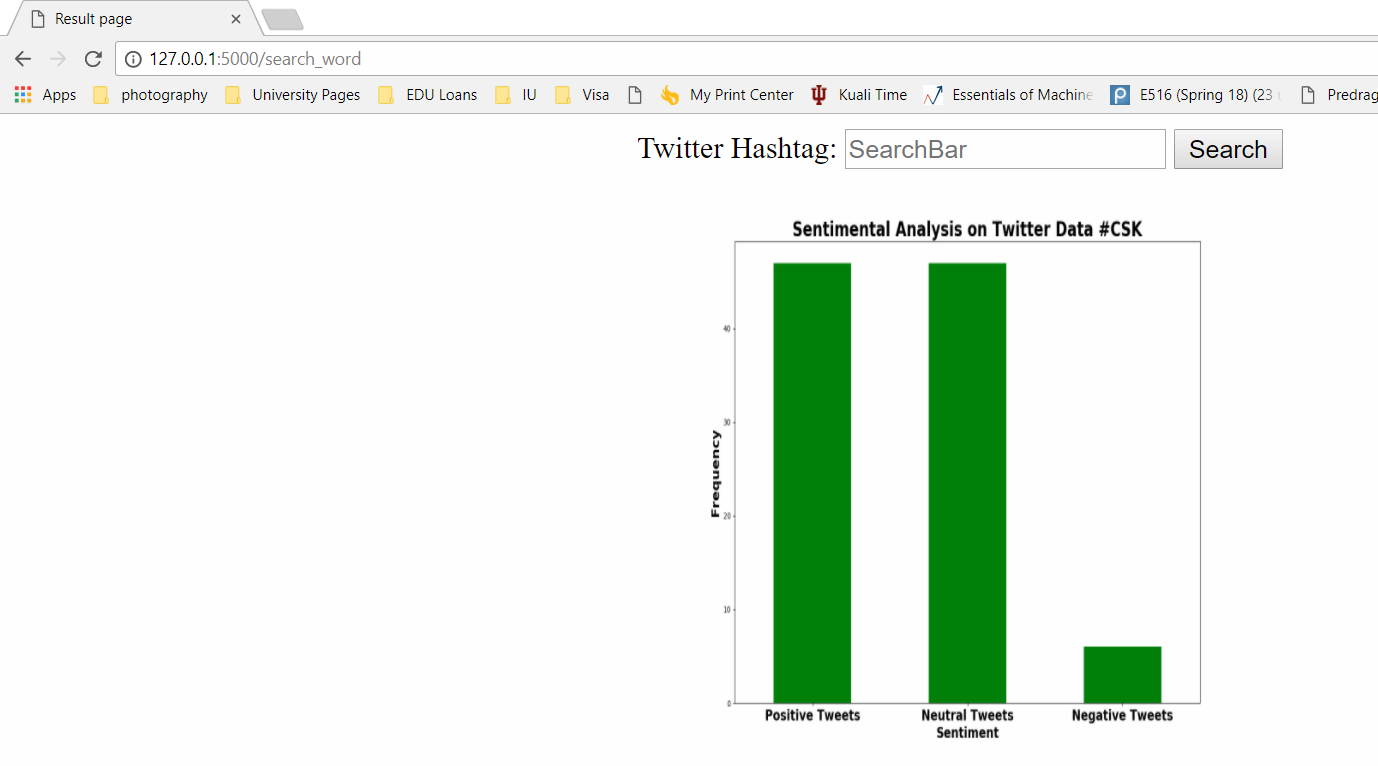
\includegraphics[width=\columnwidth]{../images/result.png}
\caption{Tweet Sentimental Classification}
\label{f:Sentimental Analysis}
\end{figure}

The above plot shows 3 different bars, first bar is for frequency of positive 
tweets, second bar is for neutral tweets and third bar is for negative tweets. 
Neutral tweets are as frequent as positive tweets but negative tweets are very 
less compared to the other two categories. This is based on the sample of the 
data we collected from the MeToo movement which comprises of roughly around 
10000 tweets. It has been in the news that as more and more victims came 
out sharing their experience through this movement, more guilty people were 
exposed and a positive sentiment is observed from majority of the people 
towards the movement lately. 


\subsection{Logistic Regression}
Logistic regression falls under the category of supervised learning. It measures 
the relationship between the categorical dependent variable and one or more independent 
variables by estimating probabilities using a logistic/sigmoid function. In spite 
of its name this is not used for regression problem where the task is to predict the 
real-valued output. Logistic regression is a bit similar to the linear regression or we 
can see it as a generalized linear model. In linear regression, we predict a 
real-valued output y based on a weighted sum of input variables. 
Logistic regression makes predictions using probability.  The name multinomial logistic 
regression refers to a case when the dependent variable has three or more unique values, 
such as Positive, Neutral, or Negative. Although the type of data used for the dependent 
variable is different from that of multiple regression, the practical use of the procedure 
is similar. Logistic regression is a powerful tool, allowing multiple explanatory 
variables being analyzed simultaneously, meanwhile reducing the effect of confounding factors. 
However, we must pay attention to model building, avoiding just feeding software 
with raw data and going forward to results ~\cite{hid-sp18-418-regression}. 
Some difficult decisions on model building will depend entirely on the expertise in 
the field of sentimental analysis.

\begin{enumerate}
\item \textbf{0 - } 
Indicates that the tweet is Neutral
\item \textbf{1 - } 
Indicates that the tweet is Positive
\item \textbf{2 - } 
Indicates that the tweet is Negative

\subsection{Spark}
``Apache Spark is a fast, in-memory data processing engine with elegant and expressive 
development APIs to allow data workers to efficiently execute streaming, machine 
learning or SQL workloads that require fast iterative access to datasets, with spark running 
on Apache Hadoop YARN, developers everywhere can now create applications 
to exploit Spark’s power, derive insights, and enrich their data science workloads 
within a single, shared dataset in Hadoop''~\cite{hid-sp18-418-spark}. Apache Spark comprises 
of Spark Core and a repository of libraries. The core of spark is the distributed execution 
engine and Python APIs offer a platform for distributed ETL application development. There are many 
libraries built on top of the core which support extensive machine learning operations.

\subsection{Spark MLlib}
MLlib is apache spark's inbuilt machine learning library, it is highly scalable. 
``MLlib fits into Spark's APIs and interoperates with NumPy in Python (as of Spark 0.9) 
and R libraries (as of Spark 1.5) '' ~\cite{hid-sp18-418-sparkml}.``We can use any Hadoop data source 
(HDFS, HBase, or local files), making it easy to plug into Hadoop workflows '' ~\cite{hid-sp18-418-sparkml}. 
MLlib has a huge repository of Machine Learning Algorithms including classification algorithms, 
Regression algorithms, Decision tree algorithms, Clustering algorithms, topic modeling algorithms and 
so on. In our project we have used the multinomial logistic regression classifier from the Spark MLlib. The MLlib 
is also capable of feature transformations, pipleline construction, parameter tuning, model evaluation and 
so on. ``MLlib contains high-quality algorithms that leverage iteration, 
and can yield better results than the one-pass approximations sometimes used 
on MapReduce '' ~\cite{hid-sp18-418-sparkml}. Spark MLlib also has libraries that can 
do feature engineering related tasks like dimensionality reduction and so on, just in case 
the number of features that are being used to build the model turns out to be really high and 
we would need to scale it to construct an efficient model.

\subsection{Spark ML Pipeline}
Pipelining is a type of architectural technique used in data science related projects. 
It is the process of collecting the instructions from the processor through a well defined 
pipeline. It enables us to execute and store commands in an organized manner. This operation is also known as 
pipeline processing. Pipelining is a technique where multiple commands are 
stacked upon each other during execution. Pipeline is divided into numerous stages and all these stages 
are connected within themselves to form a pipe like structure. The commands enter 
from one end and exit from the other end. Pipelining the process increases the overall throughput of the task at hand.//

\begin{figure}[!ht]
\centering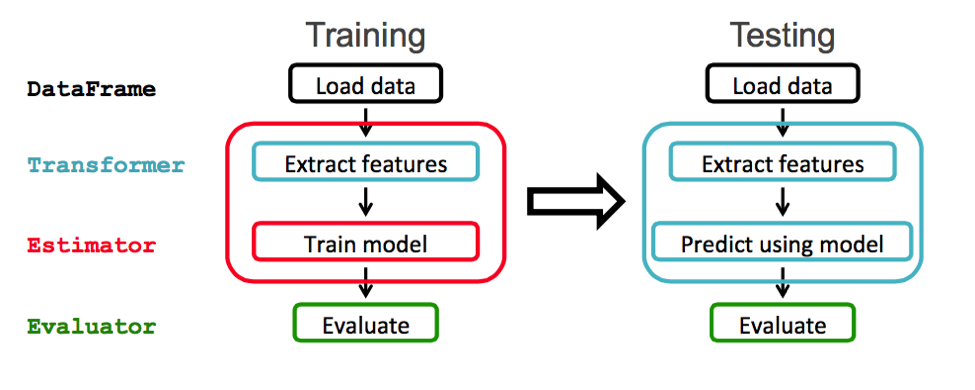
\includegraphics[width=\columnwidth]{../images/spark_pipeline.png}
\caption{SparkML Pipeline~\cite{hid-sp18-418-spark-pipeline}}
\label{f:Pipeline in SparkML}
\end{figure}

The pipeline feature available at Spark ML Pipleline is a type of high level abstraction which helps 
in modeling of a entire data science project. The ML pipeline package available in the Spark ML models a 
typical data science oriented workflow and it provides overall abstractions like Transformer, Estimator, 
Pipeline & Parameters ~\cite{hid-sp18-418-spark}. This is an overall general abstraction 
layer that makes the analysis part more productive.

\subsection{Docker}
Docker is the company driving the container movement. Docker provides a container 
platform to address every application across the hybrid cloud. 
``Today’s businesses are under pressure to digitally transform but are constrained 
by existing applications and infrastructure while rationalizing an increasingly 
diverse portfolio of clouds, datacenters and application architectures, but Docker 
enables true independence between applications and infrastructure and developers 
and IT ops to unlock their potential and creates a model for better collaboration 
and innovation'' ~\cite{hid-sp18-418-docker}. A container platform allows solving 
multiple problems across a diverse range of applications. Container platforms deliver sustainable benefits 
throughout a community by providing enterprise application modules including security, governance, 
automation, support and certification over the entire application lifecycle ~\cite{hid-sp18-418-docker}.

\section{Results}

\section{Conclusion}

\section{Work Breakdown}
Surya Prakash Sekar has worked on the python code to pre-process and clean the entire dataset 
obtained, feature extraction, build the sentimental analysis classifier model and to visualize the results on graph using 
matplotlib. Venkatesh Aditya has worked on the feature engineering for the model ,the spark code to 
build the multinomial logistic regression model that classifies the sentiment on the tweets.
The RESTful webservice was collectively done by both Venkatesh Aditya and Surya Prakash Sekar. 
The report work was collectively done by both Venkatesh Aditya and Surya Prakash Sekar as well.

\begin{acks}

	The authors would like to thank Dr.~Gregor~von~Laszewski for his
	support throughout the project and suggestions to write this paper.

\end{acks}


\bibliographystyle{ACM-Reference-Format}
\bibliography{report} 
